\documentclass[a4paper, fontsize = 14pt]{article}
\usepackage{hyperref}
\usepackage[warn]{mathtext}
\usepackage[english,russian]{babel}
\usepackage[utf8x]{inputenc} 
 
%математика
\usepackage{eucal}
\usepackage{amsmath,amsfonts,amssymb,amsthm,mathtools}
\usepackage{icomma}
\usepackage{wasysym}
\usepackage{mathrsfs}
 
%оформление текста
\usepackage{setspace}
\onehalfspacing
\usepackage{indentfirst}
\usepackage{scrextend}
 
%геометрия
\usepackage{geometry}
\geometry{left=25mm,right=25mm,
 top=25mm,bottom=30mm}
 
%графика
\usepackage{wrapfig}
\usepackage{graphicx}
\usepackage{pgfplots}
\usepackage{tikz}
\RequirePackage{caption}
\DeclareCaptionLabelSeparator{defffis}{ --- }
\captionsetup{justification=centering,labelsep=defffis}
 
%таблицы
\usepackage{array,tabularx,tabulary,booktabs} 
\usepackage{longtable}  
\usepackage{multirow} 
 
%ссылки
\usepackage{hyperref}
\usepackage{xcolor}
\definecolor{grn}{HTML}{57A14F} %зеленый
\definecolor{rd}{HTML}{E53C44} %красный 
\definecolor{bl}{HTML}{282691} %синий 
\definecolor{bbl}{HTML}{001B6C} %темно-синий
\hypersetup{		
    colorlinks=true,       	
    linkcolor=bbl,          % внутренние ссылки
    citecolor=rd,          % на библиографию
    filecolor=magenta,      % на файлы
    urlcolor=bl           %внешние источники
}
 
% Колонтитулы
\usepackage{fancyhdr} 
 	\pagestyle{fancy}
 	\renewcommand{\headrulewidth}{0.15mm}  
 	\renewcommand{\footrulewidth}{0.15mm}
 	\lfoot{МФТИ, 2021}
 	\rfoot{\thepage}
 	\cfoot{}
 	\rhead{}
 	\chead{}
 	\lhead{}
 
 
\begin{document}

\begin{center} \textbf{
Лабораторная работа №4.8 \\ Резонанс напряжений \\ 
Мещеряков Всеволод, Б02-001, 13.10.2021}
\end{center} 

\subsection*{Введение}

Цель работы заключается в изучении последовательной цепи переменного тока и наблюдении резонанса напряжений. Для этого используются регулировочный автотрансформатор, катушка индуктивности с выдвижным сердечником, магазин емкостей, резисторы, амперметр, три вольтметра, ваттметр, осциллограф, универсальный мост.

\subsection*{Теоретическая справка: импеданс}

Параметры основных элементов цепи задаются их импедансами, то есть некоторыми комплексными числами. Такая условность носит название метода "комплексных амплитуд". Поймем, в чем заключается выгода такого приёма.

Рассмотрим стандартный RLC-контур, подключенный к источнику внешней ЭДС, изменяющейся по гармоническому закону: $\varepsilon = \varepsilon_0 \cos{\Omega t}$. Обозначим разность потенциалов на конденсаторе $U_c$, ток, идущий в контуре, $I$. Сумма падений напряжения на элементах цепи равна ЭДС самоиндукции плюс ЭДС источника:

\begin{equation}
	RI + U_c = -L \frac{dI}{dt} + \mathcal{E}_0 \cos{\Omega t}.
\end{equation}

Пусть на конденсаторе заряд q, учтем зависимость от времени $q = \int I dt$:

\begin{equation}
	L \frac{dI}{dt} + RI + \frac{1}{C} \int I dt = \varepsilon_0 \cos{\Omega t}.
\end{equation}

Решением линейного этого ДУ состоит из общего однородного решения и какого либо частного решения уравнения с учетом правой части. Для поиска этого решения используется метод комплексной амплитуды: пусть некоторая комплексная функция является решением линейного ДУ с вещественными коэффициентами и комплексной правой частью; тогда вещественная часть этой функции является решением этого же уравнения, в правой части которого стоит вещественная часть прежнего выражения, а мнимая часть -- решением уравнения с мнимой частью. Исходя из сказанного, запишем уравнение (2) в комплексной форме:

\begin{equation}
	L \frac{d \hat{I}}{dt} + R\hat{I} + \frac{\int \hat{I} dt}{C} = \hat{\varepsilon_0} e^{i \Omega t}.
\end{equation}

Здесь $\hat{\varepsilon_0}$ -- комплексная амплитуда внешнего напряжения: $\hat{\varepsilon_0} = \varepsilon_0 e^{i \varphi}$. 

Если начальная фаза равна нулю, то $\hat{\varepsilon_0} = \varepsilon_0$. Правая часть (2) является вещественной частью правой части (3). Будем искать решение (3) в том же виде, что и ЭДС. Тогда получим:

\begin{equation}
	\hat{I_0}[R+i(\Omega L - \frac{1}{\Omega C})] = \varepsilon_0.
\end{equation}

Величина, стоящая в квадратных скобках, называется импедансом -- это характеристика контура, не зависящая ни от токов, ни от напряжений. Выражение (4) является обобщением законом Ома для переменных токов. Действительная часть импеданса называется активным сопротивлением контура, а мнимая -- реактивным сопротивлением контура или реактансом. Так импеданс индуктивности равен $i\Omega L$, емкости $\frac{1}{i \Omega L}$, сопротивления R.

Вернемся к началу выкладок и скажем, что фаза ЭДС не равна нулю:

\begin{equation}
	\varepsilon = \varepsilon_0 \cos{\Omega t + \varphi}.
\end{equation}

Решаем аналогичные уравнения, обозначаем импеданс Z:

\begin{equation}
	\hat{\varepsilon_0} = Z \hat{I_0}.
\end{equation}

Тогда получаем окончательно:

\begin{equation}
	I = \frac{\varepsilon_0}{|Z|} \cos{(\Omega t + \varphi - \psi)},
\end{equation}

где $\psi = arctg\frac{\Omega L - \frac{1}{\Omega C}}{R}$. 

То есть получили, что ток отстаёт от напряжения по фазе на величину $\psi$, определяемую отношением мнимой и действительной частью импеданса. 

\subsection*{Теоретическая справка: измерения}

Рассмотрим электрическую цепь, состоящую из резистора R и катушки индуктивности L с импедансом $Z_L = r_L + i\Omega L$, последовательно подключенных ко внешнему источнику, ЭДС которого меняется по синусоидальному закону с частотой $\Omega$ -- рисунок 1.

\begin{figure}[hbt]
	\centering
	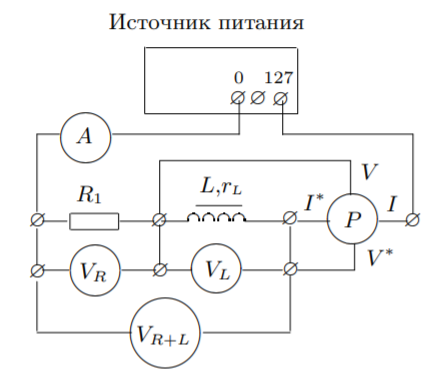
\includegraphics[scale=1]{lab48ris1.png}
	\caption{Схема экспериментальной установки для изучения закона Ома в цепи переменного тока}
\end{figure}

Обозначим через $U_R$ напряжение на резисторе, $U_L$ -- на катушке, $U_{R+L}$ -- суммарное напряжение на катушке и на резисторе. Для них справедливы комплексные выражения:

\begin{equation}
	\hat{U}_R = \hat{I} R, \,\, \hat{U}_L = \hat{I}(r_L + i\Omega L), \,\, \hat{U}_{R+L} = \hat{I}(R + r_L + i\Omega L).
\end{equation}

\text{ } \\ 

Переходя к модулям и фазам токов, получаем:

\begin{table}[hbt]
\centering
\begin{tabular}{cc}
$U_R = I \cdot R$                              & $tg \psi_1 = 0$                        \\
$U_L = I \sqrt{{r^2}_L+(\Omega L)^2}$         & $tg \psi_2 = \frac{\Omega L}{r_L}$     \\
$U_{R+L} = I \sqrt{(R+r_L)^2 + (\Omega L)^2}$ & $tg \psi_3 = \frac{\Omega L}{R + r_l}$
\end{tabular}
\end{table}

Рассчитаем среднюю мощность переменного тока, выделяемую в катушке:

\begin{equation}
	\bar P = \frac{1}{T} \int_0^T U(t) I(t) dt = I^2 r_L. 
\end{equation}

Активное сопротивление катушки $r_L$ можем измерить, если включим катушку в последовательный контур с известными $R$ и $C$ -- рисунок 2. В контуре, настроенном в резонанс на частоту $\Omega$ внешнего источника (собственная частота контура и внешняя совпадают: $\omega_0 = \Omega$), реактивные сопротивления индуктивности совпадают:

\begin{equation}
	\omega_0 L = \frac{1}{\omega_0 C}. 
\end{equation}

Тогда, определив каким либо образом добротность контура $Q$, можно рассчитать полное сопротивление контура $R_{\sum}$ в резонансе, поскольку:

\begin{equation}
	Q = \frac{\omega_0 L}{R_{\sum}} = \frac{1}{\omega_0 C R_{
	\sum}}. 
\end{equation}

\begin{figure}[hbt]
	\centering
	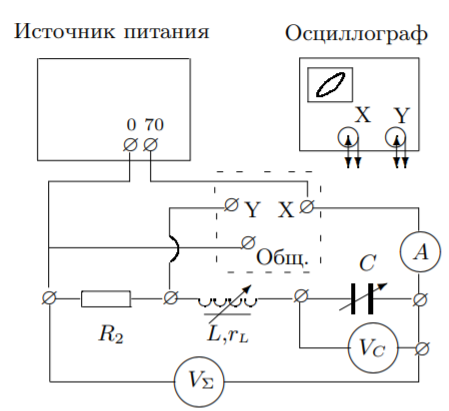
\includegraphics[scale=0.8]{lab48ris2.png}
	\caption{Схема установки для наблюдения резонанса напряжений}
\end{figure}

\subsection*{Ход работы: закон Ома}

Подготовим к работе установку, собранную по схеме рисунка 1. Перемещая сердечник катушки малыми шагами по 0.2 мм снимем зависимость тока $I$, напряжений $U_R$, $U_L$, $U_{R+L}$ и мощности $P_L$ от координаты сердечника $x$. Результаты отразим в таблице 1. Учтем и погрешности: класс точности используемых приборов -- 0,5. То есть погрешность -- $0,5\%$ от предела измерений. 

\begin{table}[hbt]
\centering
\scalebox{0.7}{
\begin{tabular}{|c|c|c|c|c|c|c|c|c|c|c|}
\hline
\textbf{$x, мм$} & \textbf{$I, дел$} & \textbf{$\sigma_I, дел$} & \textbf{$U_R, дел$} & \textbf{$\sigma_{U_R}, дел$} & \textbf{$U_{R+L}, дел$} & \textbf{$\sigma_{U_{R+L}}, дел$} & \textbf{$U_{L}, дел$} & \textbf{$\sigma_{U_L}, дел$} & \textbf{$P_L, дел$} & \textbf{$\sigma_{P_L}, дел$} \\ \hline
5,00             & 29                & 0,01                     & 63                  & 1                            & 118                     & 1                                & 89                    & 1                            & 52                  & 0,125                        \\ \hline
7,00             & 34                & 0,01                     & 73                  & 1                            & 116                     & 1                                & 79                    & 1                            & 47                  & 0,125                        \\ \hline
9,00             & 36                & 0,01                     & 80                  & 1                            & 114                     & 1                                & 71                    & 1                            & 43                  & 0,125                        \\ \hline
11,00            & 38                & 0,01                     & 83                  & 1                            & 113                     & 1                                & 64                    & 1                            & 40                  & 0,125                        \\ \hline
13,00            & 39                & 0,01                     & 87                  & 1                            & 112                     & 1                                & 59                    & 1                            & 38                  & 0,125                        \\ \hline
15,00            & 40                & 0,01                     & 89                  & 1                            & 111                     & 1                                & 55                    & 1                            & 36                  & 0,125                        \\ \hline
17,00            & 41                & 0,01                     & 90                  & 1                            & 110                     & 1                                & 52                    & 1                            & 34                  & 0,125                        \\ \hline
19,00            & 41                & 0,01                     & 91                  & 1                            & 110                     & 1                                & 49                    & 1                            & 33                  & 0,125                        \\ \hline
21,00            & 42                & 0,01                     & 92                  & 1                            & 109                     & 1                                & 46                    & 1                            & 31                  & 0,125                        \\ \hline
\end{tabular}
}
\caption{Результаты измерений до пересчёта, значения указаны в делениях приборов}
\end{table}

Пересчитаем деления в соответствующие единицы измерения. Амперметр выставлен на максимальный ток 2.5 А, имеет 100 делений -- тогда 1 деление -- это 0,025 A. Вольтметры выставлены на максимальное напряжение 150 В, имеют 150 делений -- тогда 1 деление -- это 1 В. Ваттметр, согласно документации, показывает 1 Вт на деление. Результаты укажем в таблице 2.

\begin{table}[hbt]
\centering
\scalebox{0.8}{
\begin{tabular}{|c|c|c|c|c|c|c|c|c|c|c|}
\hline
\textbf{$x, мм$} & \textbf{$I, А$} & \textbf{$\sigma_I, A$} & \textbf{$U_R, В$} & \textbf{$\sigma_{U_R}, В$} & \textbf{$U_{R+L}, В$} & \textbf{$\sigma_{U_{R+L}}, В$} & \textbf{$U_{L}, В$} & \textbf{$\sigma_{U_L}, В$} & \textbf{$P_L, Вт$} & \textbf{$\sigma_{P_L}, Вт$} \\ \hline
5                & 0,73            & 0,03                   & 63                & 1                          & 118                   & 1                              & 89                  & 1                          & 13                 & 0,03                        \\ \hline
7                & 0,85            & 0,03                   & 73                & 1                          & 116                   & 1                              & 79                  & 1                          & 12                 & 0,03                        \\ \hline
9                & 0,90            & 0,03                   & 80                & 1                          & 114                   & 1                              & 71                  & 1                          & 11                 & 0,03                        \\ \hline
11               & 0,95            & 0,03                   & 83                & 1                          & 113                   & 1                              & 64                  & 1                          & 10                 & 0,03                        \\ \hline
13               & 0,98            & 0,03                   & 87                & 1                          & 112                   & 1                              & 59                  & 1                          & 10                 & 0,03                        \\ \hline
15               & 1,00            & 0,03                   & 89                & 1                          & 111                   & 1                              & 55                  & 1                          & 9                  & 0,03                        \\ \hline
17               & 1,03            & 0,03                   & 90                & 1                          & 110                   & 1                              & 52                  & 1                          & 9                  & 0,03                        \\ \hline
19               & 1,03            & 0,03                   & 91                & 1                          & 110                   & 1                              & 49                  & 1                          & 8                  & 0,03                        \\ \hline
21               & 1,05            & 0,03                   & 92                & 1                          & 109                   & 1                              & 46                  & 1                          & 8                  & 0,03                        \\ \hline
\end{tabular}
}
\caption{Результаты измерений после пересчёта, значения указаны в соответствующих единицах измерения}
\end{table}

По формуле для $U_L$ из (8) и формуле (9) рассчитаем $r_L$ и $L$ для каждого $x$.  Оценим погрешности: $\sigma_x = 0.5 мм$, $\sigma_{r_L}$ как косвенное измерение через погрешности $P$ и $I$. Результаты отразим в таблицах 3 и 4, по ним построим графики на рисунках 3 и 4.

Оценка погрешностей в этой работе несет условный характер, так как провода и клеммы вносят неоценимый вклад. Для реактивного сопротивления удалось провести оценку, но для индуктивности адекватной оценки провести не удалось.

\begin{table}[hbt]
\centering
\begin{tabular}{|c|c|c|c|}
\hline
\textbf{$x, мм$} & \textbf{$\sigma_x, мм$} & \textbf{$r_l, Ом$} & \textbf{$\sigma_{r_l}, Ом$} \\ \hline
5                & 0,5                     & 12,37              & 2,13                        \\ \hline
7                & 0,5                     & 8,13               & 1,20                        \\ \hline
9                & 0,5                     & 6,64               & 0,92                        \\ \hline
11               & 0,5                     & 5,54               & 0,73                        \\ \hline
13               & 0,5                     & 5,00               & 0,64                        \\ \hline
15               & 0,5                     & 4,50               & 0,56                        \\ \hline
17               & 0,5                     & 4,05               & 0,49                        \\ \hline
19               & 0,5                     & 3,93               & 0,48                        \\ \hline
21               & 0,5                     & 3,51               & 0,42                        \\ \hline
\end{tabular}
\caption{Точки для графика зависимости $r_L(x)$}
\end{table}

\begin{table}[hbt]
\centering
\begin{tabular}{|c|c|c|}
\hline
\textbf{$x, мм$} & \textbf{$\sigma_x, мм$} & \textbf{$L, Гн$} \\ \hline
5                & 0,5                     & 0,39             \\ \hline
7                & 0,5                     & 0,29             \\ \hline
9                & 0,5                     & 0,25             \\ \hline
11               & 0,5                     & 0,21             \\ \hline
13               & 0,5                     & 0,19             \\ \hline
15               & 0,5                     & 0,17             \\ \hline
17               & 0,5                     & 0,16             \\ \hline
19               & 0,5                     & 0,15             \\ \hline
21               & 0,5                     & 0,14             \\ \hline
\end{tabular}
\caption{Точки для графика зависимости $L(x)$}
\end{table}

\begin{figure}
	\centering
	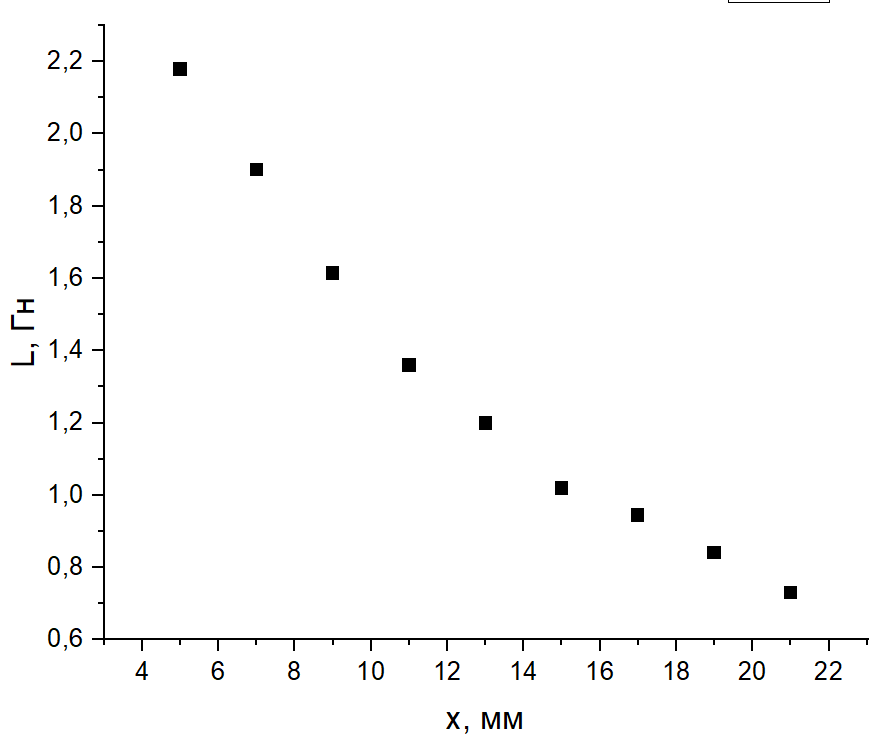
\includegraphics[scale=0.7]{lab48ris4.png}
	\caption{График зависимости $r_L(x)$}
\end{figure}

\begin{figure}
	\centering
	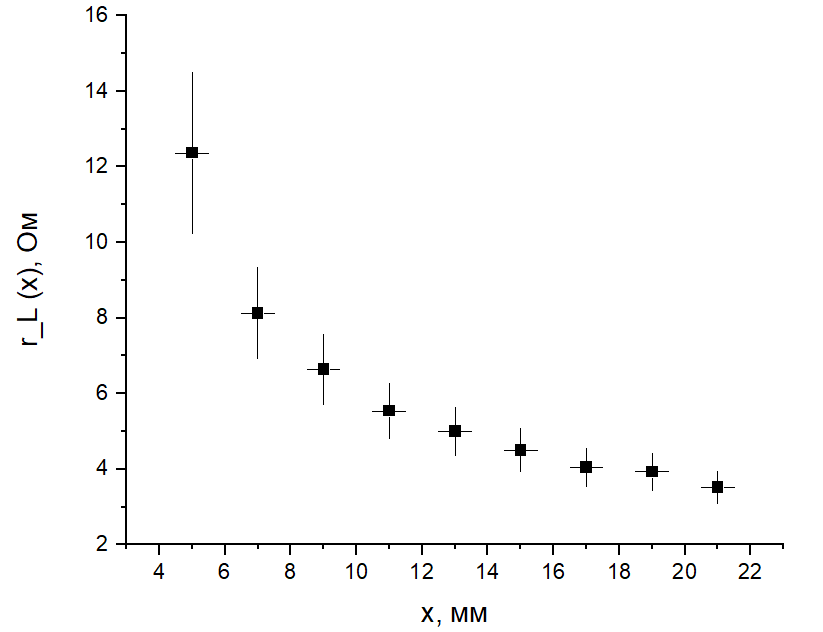
\includegraphics[scale=0.7]{lab48ris3.png}
	\caption{График зависимости $L(x)$}
\end{figure}

\newpage

Теперь построим векторную диаграмму (Рис. 5) напряжений. Напряжение на резисторе совпадает по фазе с током, поэтому $U_R$ лежит на векторе $I$. Векторное равенство напряжений $U_{L+R} = U_L + U_R$ позволяет построить треугольник по трем сторонам. Сделаем две насечки: первую -- радиусом, равным модулю вектора $U_{R+L}$, из начала вектора $U_R$ (см. схему на Рис. 1); вторую -- радиусом, равным модулю вектора $U_L$, из конца вектора $U_R$. Точка на пересечении насечек определяет положение векторов $U_{L+R}$ и $U_L$ на диаграмме. Разложим $U_L$ по осям координат. Проекция $U_L$ на ось $I$ равна $U_{L, акт}$, проекция на перпендикулярную ось -- $U_{L, реакт}$. 

Будем брать значения при $x = 21 \, мм$: $U_{L+R} = 109 \, В$, $U_L = 46 \, В$, $U_R = 92 \, В$. Тогда запишем теорему косинусов для получившегося треугольника напряжений, из нее получим значение угла $\beta = 81 ^\circ$, которое оказывается близким к рассчетному $83 ^\circ$.

\begin{figure}[hbt]
	\centering
	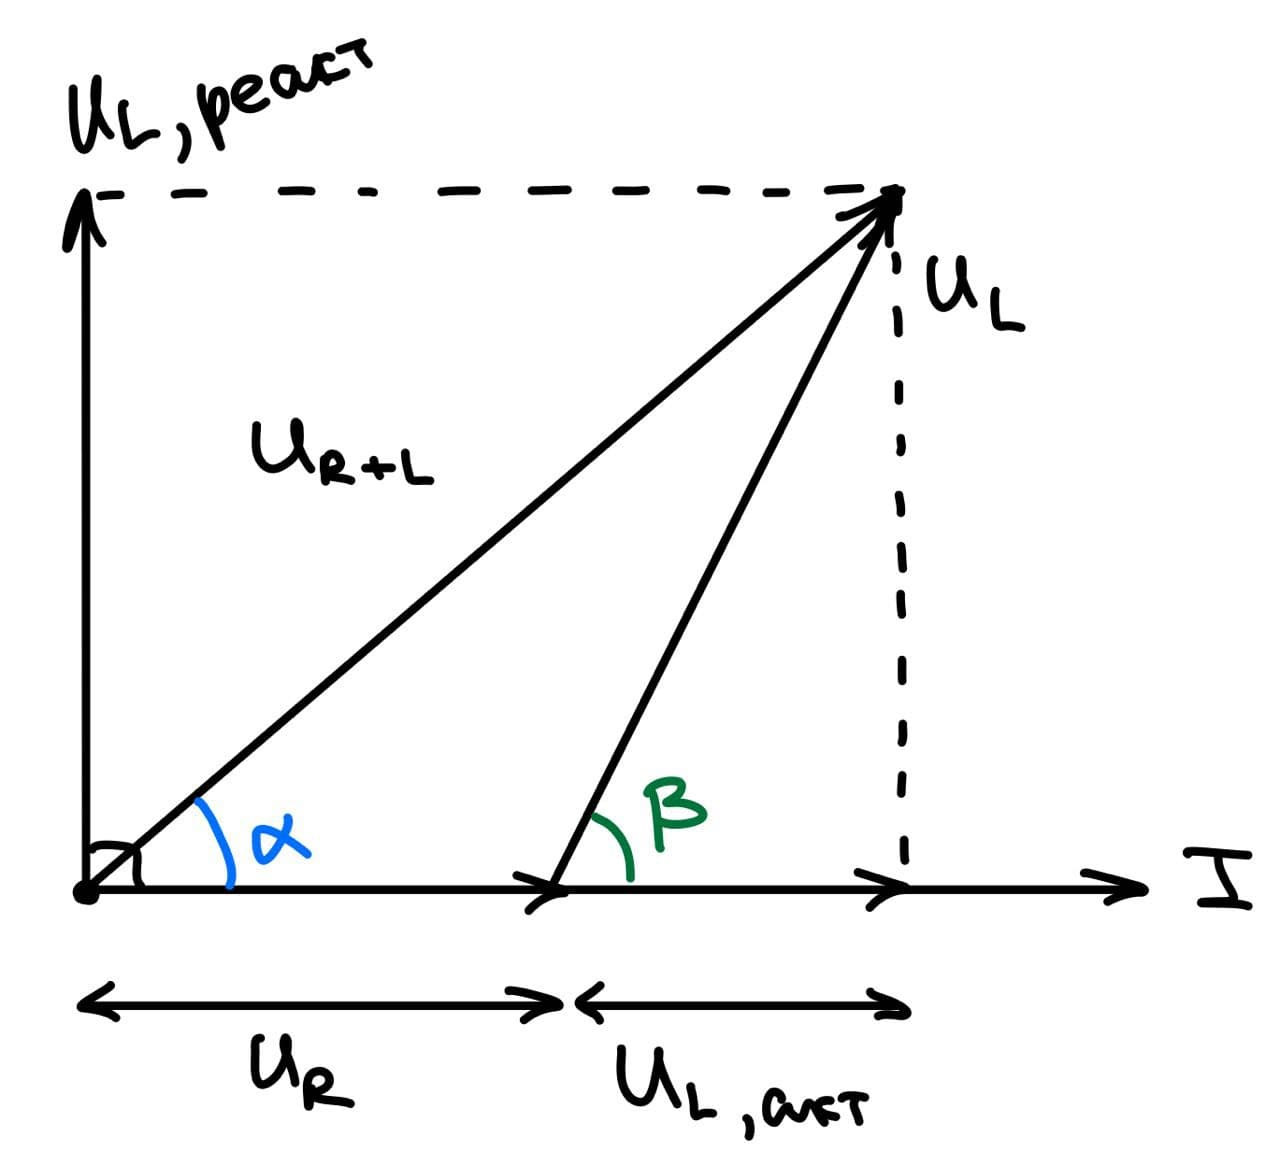
\includegraphics[scale=0.2]{lab48ris5.png}
	\caption{Векторная диаграмма}
\end{figure}

Воспользуемся методом трех вольтметров для вычисления мощности, выделяющейся на катушке при среднем положении сердечника. Записав теорему косинусов, получим: $P_L = U_L I \cos{\beta} = 8,4 \, Вт$, что оказывается близким к измеренным $10 \, Вт$ (см. Таблица 2, строка для 13 мм). 

\newpage

\subsection*{Ход работы: резонанс напряжений}

Теперь подключим катушку к установке, схема которой изображена на рисунке 2. Будем менять ёмкости и искать такое положение сердечника, чтобы катушка входила в резонанс с сетью. Критерием для нас будет являться картина, которую мы видим на экране осциллографа -- в резонансе кривые "слипляются" (см. Рис. 6).

\begin{figure}[hbt]
	\centering
	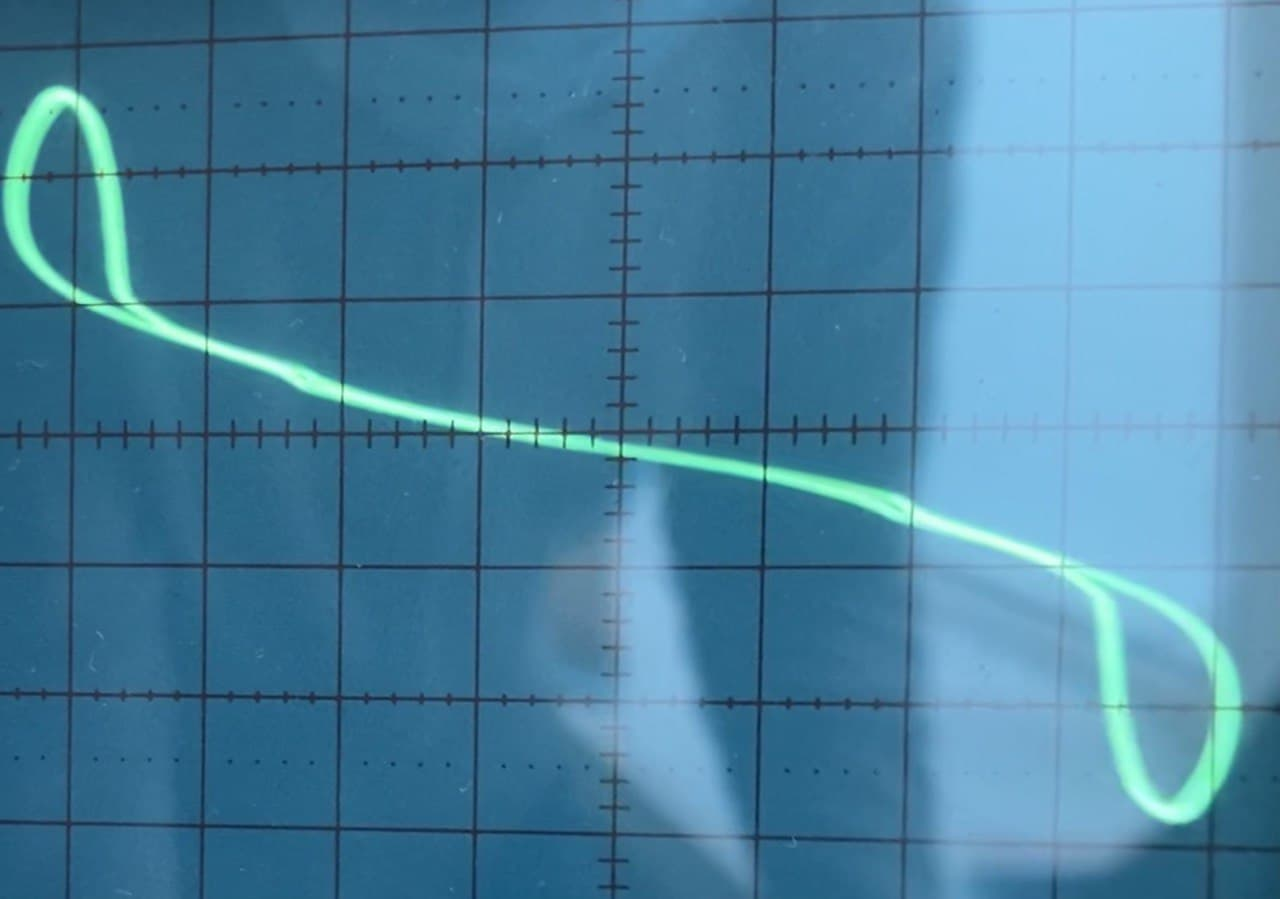
\includegraphics[scale=0.3]{lab48ris6.png}
	\caption{Кривые на осциллографе сошлись в одну -- наступил резонанс}
\end{figure}

Выберем для анализа наибольшую из измеренных ёмкостей: $C = 50,2 \pm 2,5\, мкФ$. Подберем положение сердечника такое, чтобы картина на осциллографе соответствовала резонансу. Для выбранной ёмкости это $x = 11 \pm 0.5$. Снимем показания датчиков: ток в цепи -- $I_{рез} = 4,40 \pm 0,3 \, А$,напряжение на конденсаторе $U_{C, рез} = 284\pm2 \, В$,напряжение на последовательном соединении $U_{\sum} = 43,5 \pm 2 \, В$. Тогда добротность контура можно оценить как:

\begin{equation}
	Q = \frac{U_{C, рез}}{U_{\sum, рез}} = 6,53 \pm 0,06 
\end{equation}

\end{document}